% figure: 自控-闭环负反馈框图.png
% 用途：自控 01 第1章 —— 偏差 e=r-b 与按偏差调节（反馈控制原理）
% 构建：..\build.ps1 -File .\block-feedback-loop.tex
% 说明：旧图用通用绘图工具生成，H(s) 标签溢出方框；本图改用 TikZ，标签宽度自动
%       适配方框，字号与笔记其余插图统一。
\documentclass[border=10pt]{standalone}
\usepackage{fontspec}
\setmainfont{Cambria}
\usepackage{unicode-math}
\setmathfont{Cambria Math}
\usepackage{tikz}
\usetikzlibrary{positioning, arrows.meta, calc}
\usepackage{ctex}

\definecolor{figink}{HTML}{1E2228}
\definecolor{figacc}{HTML}{B23020}
\definecolor{figfill}{HTML}{E8EFF8}
\definecolor{figsub}{HTML}{606874}

\begin{document}
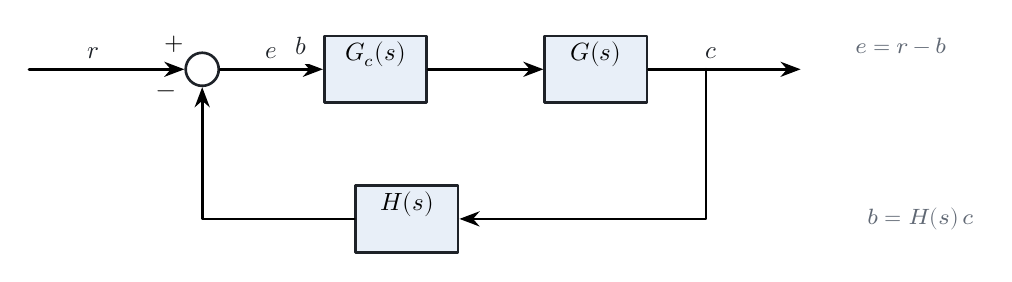
\begin{tikzpicture}[
  x=1cm, y=1cm,
  line width=0.95pt, line cap=round, line join=round,
  >=Stealth,
  blk/.style = {draw=figink, line width=0.95pt, fill=figfill,
                minimum width=1.3cm, minimum height=0.85cm, inner sep=2pt,
                anchor=center, font=\small, align=center},
  sum/.style = {draw=figink, line width=0.95pt, circle, inner sep=0pt,
                minimum size=0.42cm, anchor=center},
  sig/.style = {font=\small, color=figink, fill=white},
  lbl/.style = {font=\small, inner sep=1.5pt, fill=white},
  sub/.style = {font=\footnotesize, color=figsub, fill=white}
]

\node[sum] (s1) at (0,0) {};
\node[blk] (gc) at (2.2,0) {$G_c(s)$\\[2pt]{\footnotesize 控制器}};
\node[blk] (g)  at (5.0,0) {$G(s)$\\[2pt]{\footnotesize 被控对象}};
\node[blk] (h)  at (2.6,-1.9) {$H(s)$\\[2pt]{\footnotesize 测量反馈}};

% 前向通道
\draw[->] (-2.2,0) -- node[sig, above] {$r$（给定）} (s1.west);
\draw[->] (s1.east) -- node[sig, above] {$e$} (gc.west);
\draw[->] (gc.east) -- (g.west);
\draw[->] (g.east) -- node[sig, above] {$c$（输出）} (7.6,0);

% 反馈通道
\draw[->] (6.4,0) -- (6.4,-1.9) -- (h.east);
\draw[->] (h.west) -- (0,-1.9) -- (s1.south);

\node[lbl] at (-0.36,0.32) {$+$};
\node[lbl] at (-0.46,-0.32) {$-$};
\node[sig] at (1.25,0.30) {$b$};

% 标注
\node[sub, anchor=west] at (7.9,0.30) {偏差 $e=r-b$};
\node[sub, anchor=west] at (7.9,-1.90) {反馈信号 $b=H(s)\,c$};

\end{tikzpicture}
\end{document}
